\documentclass[12pt,oneside,a4paper]{article}

\usepackage[backend=biber,style=numeric]{biblatex}
\usepackage{xcolor}
\usepackage{todonotes}
\usepackage{amsmath}
\usepackage{multicol}
\usepackage{caption}
\usepackage{hyperref}
\usepackage{amssymb}
\usepackage{graphicx}
\usepackage{listings}
\usepackage[section]{placeins}
\lstdefinestyle{qasm}{
    belowcaptionskip=1\baselineskip,
    frame=top,frame=bottom,
    frameround=tttt,
    xleftmargin=\parindent,
    basicstyle=\footnotesize\ttfamily,
    tabsize=2,
    numbers=left,
    numbersep=5pt,
    stepnumber=1,
    columns=fullflexible,
}
\lstset{
	frame=top,frame=bottom,
	language=C,
	basicstyle=\small\normalfont,
	xleftmargin=\parindent,
	keywordstyle=\color{green!40!black},
    % FIXME remove this comments
	%  commentstyle=\itshape\color{purple!40!black},
	%  identifierstyle=\color{blue},
	%  stringstyle=\color{orange},
	morekeywords={in, globaldata, procedure, input, output, behavior, end, XOR, NOT, AND}, % keyword to highlight
	tabsize=2,
	numbers=left,
	stepnumber=1,                   % the step between two line-numbers.
	numbersep=5pt,
	framexleftmargin=10pt,
	title=\lstname,
	captionpos=t,
	showspaces=false,
}
\DeclareCaptionFormat{listing}{\rule{\dimexpr\textwidth\relax}{0.4pt}\par\vskip1pt#1#2#3}
\captionsetup[lstlisting]{format=listing,singlelinecheck=false, margin=0pt,labelsep=space,labelfont=bf}

\usepackage{booktabs}
\usepackage[noabbrev,capitalise]{cleveref}
\crefname{listing}{algorithm}{algorithms}
\Crefname{listing}{Algorithm}{Algorithms}
\renewcommand\lstlistingname{Algorithm}
\def\lstlistingcrefname{Algorithm}
\usepackage{url}

\addbibresource{assets/biblio.bib}

\title{\textbf{Quantum Circuit Simulation: A Unified Approach to Contraction, Compilation, and Execution on Heterogeneous Architectures}}

\author{Federico Lolli, Angelo Zangari}

\date{\today}

\begin{document}

\begin{titlepage}
    \centering
    \clearpage
    \maketitle
	\thispagestyle{empty}
	\vspace*{1cm}
	\vfill
	\centering
	
\includegraphics{logo_polimi.png}
\includegraphics{logo_NECST.png}
\end{titlepage}


\begin{abstract}
    In the rapidly evolving field of quantum computing, efficient simulation of quantum circuits on classical computers remains a critical challenge. This project focuses on developing a versatile and efficient simulation toolchain for quantum circuits, emphasizing compatibility with heterogeneous hardware architectures. Our approach centers on several key innovations that we believe can enhance the simulation process. At the core of our toolchain is a custom Instruction Set Architecture (ISA) that decomposes quantum circuits into a series of schedulable instructions, utilizing fundamental mathematical operators such as tensor expansions and matrix multiplications. This abstraction allows for flexible and efficient representation of quantum operations across various hardware platforms.
    We developed a prototype FPGA accelerator with custom kernels written specifically for these two operators, as a proof-of-concept to demonstrate the potential performance benefits of our approach. Our work aims to advance the field of quantum circuit simulation by providing a novel approach, concretized in a comprehensive, extensible toolchain that can adapt to various classical computing accelerators. While our current proof-of-concept targets FPGA implementation, the architecture of our toolchain lays the groundwork for efficient quantum circuit simulation on heterogeneous computing platforms, offering a powerful tool for researchers and developers in quantum computing.
\end{abstract}

\newpage
\tableofcontents

\newpage

%%%%%%%%%%%%%%%%%%%%%%%%%%%%%%%%%%%%%%%%%%%%%%%%%%%% SECTION 1

\section{Introduction}

\subsection{The Quantum Computing Landscape}

In recent years, the field of quantum computing has experienced significant advancements, promising to revolutionize computational capabilities for specific classes of problems. Quantum computers have the potential to solve certain tasks exponentially faster than their classical counterparts, particularly in areas such as cryptography \cite{Shor1995PolynomialTimeAF}, optimization \cite{Farhi2014AQA}, and quantum system simulations. However, the development and verification of quantum algorithms and circuits still heavily rely on classical computing resources.

\subsection{The Role of Classical Simulation}

Classical computers play a crucial role in the development of quantum computing technologies. They are extensively used for simulating and verifying quantum circuits, which is essential for:

\begin{itemize}
    \item Debugging and testing quantum algorithms
    \item Benchmarking quantum hardware performance
    \item Exploring the behavior of quantum systems at scales currently unattainable by physical quantum devices
\end{itemize}

Currently, popular frameworks like \textbf{Qiskit} \cite{qiskit2024} provide simulation capabilities with varying levels of performance. However, as quantum circuits grow in size and complexity, there is an increasing need for more efficient simulation techniques.

\subsection{Project Objectives}

The primary goal of this project is to develop a versatile and efficient simulation toolchain for quantum circuits, with a focus on compatibility with heterogeneous hardware while maintaining user-friendliness and integration with existing frameworks. Our key objectives can be summarized as follows:

\begin{enumerate}
    \item Design a comprehensive simulation toolchain for quantum circuits that can interface with various classical computing accelerators, including GPUs and FPGAs.
    \item Ensure interoperability with established quantum computing frameworks, particularly Qiskit, to integrate seamlessly into existing quantum development workflows.
    \item Develop a flexible representation of quantum operations that can be efficiently translated to different hardware architectures.
    \item Implement a prototype FPGA accelerator as a proof-of-concept to demonstrate the potential performance benefits of our approach.
    \item Establish a foundation for future research in heterogeneous quantum circuit simulation, allowing for easy extension to other accelerator architectures.
\end{enumerate}

Through these objectives, we aim to contribute to the advancement of quantum computing research by providing a powerful simulation toolchain that leverages the capabilities of heterogeneous computing architectures.

\subsection{Our Approach}

Our approach to quantum circuit simulation involves several key points:

\begin{itemize}
    \item \textbf{Whole circuit evaluation:} We aim to evaluate the whole circuit at once and the provide the resulting matrix, thus enabling the reuse of the matrix for successive experiments.
    \item \textbf{Use of well established standards:} By adhering to the QASM standard\cite{cross2017openquantumassemblylanguage} for quantum circuit representation we ensure compatibility with widely used quantum computing frameworks like Qiskit.
    \item \textbf{Instruction Set Architecture (ISA) Design:} We developed a custom ISA that decomposes quantum circuits into a series of instructions, enabling efficient representation and execution on various hardware platforms.
    \item \textbf{Tensor Network Contraction:} By employing tensor networks to represent quantum circuits and perform optimized contractions we aim to achieve efficient simulation in terms of computational complexity and memory usage \cite{pan2023efficientquantumcircuitsimulation}.
    \item \textbf{Sparse Matrix Operations:} We chose to represent quantum gate operands as sparse matrices (in COO format) and kept this format throughout the simulation to optimize memory usage and computational efficiency. We think that leveraging the sparsity of quantum states is crucial for efficient simulation of large circuits.
    \item \textbf{Compilation in an executable format:} We designed a compilation step that transforms the optimized contraction tree into a sequence of instructions compiled in a lightweight, portable binary format, representing the optimized computation plan. We also developed an interpreter to translate this binary format into the actual OpenCL operations to be executed on the FPGA.
    \item \textbf{Dynamic Scheduling:} Based on the optimized contraction path, we developed a scheduler that dynamically orders the instructions to maximize parallelism and minimize computational overhead.
    \item \textbf{FPGA Implementation:} We develop custom kernels from scratch, optimized for tensor expansion and matrix multiplication operations for COO sparse matrices on FPGAs to showcase the potential performance of accelerated quantum circuit simulation on heterogeneous architectures.
    \item \textbf{Use of memory safe compiled languages:} We implemented the entire simulation toolchain in Rust, leveraging its memory safety features and performance characteristics to ensure robustness and efficiency, along its extendability and maintainability.
\end{itemize}

\subsection{Report Structure}

The remainder of this report is organized as follows:

\begin{itemize}
    \item Section \ref{sec:background}: Provides necessary background information on quantum computing, tensor networks, and FPGA technology.
    \item Section \ref{sec:methodology}: Describes our simulation toolchain in detail, including the ISA design, tensor network contraction methods, and FPGA implementation.
    \item Section \ref{sec:results}: Presents the performance results of our implementation, comparing it with existing simulation methods.
\end{itemize}


%%%%%%%%%%%%%%%%%%%%%%%%%%%%%%%%%%%%%%%%%%%%%%%%%%%% SECTION 2

\section{Background}
\label{sec:background}

\subsection{What is quantum computing}
Quantum computing represents a revolutionary approach to information processing, fundamentally different from classical computing. It harnesses the principles of quantum mechanics to perform calculations, offering the potential to solve certain problems exponentially faster than traditional computers.
At the heart of quantum computing are quantum bits, or qubits. Unlike classical bits that can only be in one of two states (0 or 1), qubits can exist in a superposition of states, effectively encoding multiple classical states simultaneously. This unique property allows quantum computers to process vast amounts of information in parallel.
Quantum circuits, the building blocks of quantum computation, consist of quantum gates that manipulate qubits. These circuits differ significantly from classical circuits, which use high and low voltages to represent binary states. Instead, quantum circuits leverage quantum superposition to encode and process multiple states concurrently.

\subsection{What is a quantum gate}
Quantum gates are fundamental components in quantum computing, serving as the building blocks of quantum circuits. These gates are mathematical representations of unitary operations that manipulate quantum states, analogous to logic gates in classical circuits but with significantly different properties and capabilities.
Unlike classical gates that operate on definite binary states (0 or 1), quantum gates act on qubits, which can exist in superpositions of states. This key difference allows quantum gates to perform complex quantum operations that have no direct classical counterpart.
The unitary nature of quantum gates ensures that the total probability of all possible outcomes remains conserved, a crucial property in maintaining the integrity of quantum information. These gates enable various transformations of quantum states, including rotations in the complex vector space, phase shifts, and entanglement operations between multiple qubits.
% TODO add simple drawing + explanation
Quantum circuits are constructed by combining these quantum gates in specific sequences. While classical circuits use high and low voltages to represent and process binary information, quantum circuits leverage the quantum superposition principle to encode and manipulate multiple states simultaneously. This parallel processing capability is a key factor in the potential computational advantage of quantum systems.
The implementation of quantum gates allows for the execution of complex quantum algorithms. These algorithms can perform tasks such as quantum Fourier transforms, quantum error correction, and other operations that exploit the unique properties of quantum systems.
In essence, quantum gates are the operators that drive quantum computation, enabling the manipulation and transformation of quantum information in ways that are fundamentally different from classical information processing. Their ability to act on superpositions and create entanglement is central to the power and promise of quantum computing.

\subsection{Measurement}
Measurement is a critical and unique aspect of quantum computing, fundamentally different from classical data readout. It represents the process of extracting information from a quantum system, bridging the quantum world with our classical reality.
In quantum computing, measurement involves observing the state of a qubit or a system of qubits. However, this process is not straightforward due to the probabilistic nature of quantum mechanics. When a measurement is performed, it causes the quantum state to "collapse" from a superposition of potential states into a definite classical state.
This collapse results in a binary string (bitstring) in the measurement basis, effectively converting quantum information into classical information. For example, a qubit in superposition might collapse to either '0' or '1' upon measurement, with probabilities determined by its quantum state prior to measurement.
A key characteristic of quantum measurement is its irreversibility. Once a measurement is made, the original superposition is lost, and repeated measurements on the same qubit will yield the same result. This property has profound implications for quantum algorithms and error correction techniques.
Furthermore, the probabilistic nature of quantum measurement means that a single measurement doesn't provide complete information about the original quantum state. To gain comprehensive understanding, the entire quantum computation typically needs to be repeated multiple times, with measurements performed each time. This allows for the reconstruction of the probability distribution of possible outcomes, providing insights into the quantum state before measurement.
Understanding and managing the measurement process is crucial in quantum computing. It affects how quantum algorithms are designed, how results are interpreted, and how quantum error correction is implemented. The interplay between quantum operations and measurement is a fundamental consideration in harnessing the power of quantum computation.

\subsection{Different approaches for quantum circuit simulation}
There are many different methods to tackle the simulation problem, mainly divided into two categories: state vector propagation and tensor networks.
The first method is the traditionally used one. It consists in computing the state vector of the circuit and propagating it through the circuit from the start to the end. Although method is functional, it presents severe limitations; mainly using a state vector to represent the circuit means that we need to store it, but the issue is that the vector dimension grows exponentially with respect to the number of circuit lanes. This renders the state vector method computationally infeasible from a spatial point of view for circuits with bigger dimension.
The second method is newer and resorts to decomposing the quantum circuit into its corresponding tensor network representation. From here we can perform mathematical operations to contract the terms and get an equivalent expression of the circuit.
This method presents multiple great benefits:
\begin{itemize}
    \item perform computations on subset of data, can be contained in fpga
    \item independent operations, can be scheduled in parallel
    \item decomposing in different operations allows for specific implementations (e.g. different fpga kernels)
\end{itemize}

Quantum circuit simulation is a crucial tool in quantum computing research and development. Two main approaches have emerged to tackle this challenge: state vector propagation and tensor network methods.

\subsubsection{State Vector Propagation:}
This traditional method involves computing and propagating the state vector of the circuit from start to finish. While functional, it faces severe limitations, primarily due to the exponential growth of the state vector's dimension with respect to the number of circuit lanes. This exponential scaling renders the state vector method computationally infeasible for larger circuits, especially when the number of qubits exceeds 50.

\subsubsection{Tensor Network Methods:}
A more recent approach involves decomposing the quantum circuit into its corresponding tensor network representation. This method offers several advantages:

\begin{itemize}
    \item Subset Computation: It allows for computations on subsets of data, making it feasible for implementation on devices with limited memory, such as FPGAs.
    \item Parallelization: Independent operations can be scheduled and executed in parallel, enhancing computational efficiency.
    \item Specialized Implementations: Decomposition into different operations allows for specific implementations, such as different FPGA kernels for various tensor operations.
\end{itemize}

In the tensor network approach, quantum gates and initial states are represented as tensors and vectors, respectively. The circuit's structure is mapped to bonds between these tensors, creating a unique tensor network. Contracting this network yields a vector representing the final quantum state, containing amplitudes for the entire Hilbert space.

Tensor Network Simulation Categories:
\begin{enumerate}
    \item Single Amplitude Simulation: Focuses on computing the amplitude of a single bitstring, with maximal restriction on the final state.
    \item Full State Simulation: Aims to obtain all amplitudes in the entire Hilbert space, with no restrictions on the final state. However, this is feasible only for small qubit numbers due to exponential memory requirements.
    \item Subspace Simulation: A middle ground approach, partially closing the final state and allowing direct obtainment of amplitudes for an opened Hilbert subspace.
    \item Sparse-State Simulation: Designed to calculate amplitudes of multiple bitstrings in one tensor network contraction, with specific restrictions on the final state configuration.
\end{enumerate}

The choice among these methods depends on the circuit size, available computational resources, and the specific requirements of the simulation task. Tensor network methods, particularly sparse-state simulation, offer a promising approach for simulating larger quantum circuits that are beyond the capabilities of traditional state vector methods.



\subsection{Tensor Expansion}
% TODO check, complete and expand
Is a mathematical operator through which two tensors originate a third one with rank the product of the rank of the input tensors. There are many algorithms to implement it, such as the Einsum notation, which compresses the indexes, or the kronecker product. We followed the latter, in which every element of the first matrix is multiplied by the entire second matrix and then be appropriately put in the result matrix.

\subsection{Tensor Contraction}
% TODO check, complete and expand
Can be though as a generalization of a matrix multiplication. It can be performed between two tensors with same rank and spanning on exactly the same lanes, with no other quantum gates in between. The resulting tensor has the same dimensions (rank) as the starting tensors and each element can be computed as the traditional dot product between the appropriate row and column of the first and second matrix, respectively.


\subsection{Sampling and evaluating quality of obtained sample with LXEB}
Our work poses as objective the computation of the tensor representing the final and contracted quantum circuit. This allows us to obtain a sample of the output bitstring simply by multiplying it for the input vector. After having computed the output tensor, it is useful to remark for completeness what needs to be done for the verification part of the quantum experiment. Verification is used to evaluate the quality of quantum computations. In particular, in Random Circuit Sampling (RCS) experiments, researchers use the Linear Cross-Entropy Benchmark (LXEB) to quantify the circuit quality. The LXEB serves as a proxy for fidelity in large quantum circuits where direct fidelity calculation is impractical. It compares the distribution of sampled bitstrings from the quantum device with the ideal theoretical distribution, providing a measure of how well the quantum computation aligns with expectations.

Quantum simulation on classical computers faces significant challenges due to the exponential growth of the quantum state space with the number of qubits. For instance, storing the full quantum state vector becomes infeasible for systems with more than 50 qubits. To address this, tensor network methods have emerged as a powerful tool for simulating quantum circuits. These methods represent quantum gates and states as tensors, mapping the circuit to a network of interconnected tensors. By contracting this network, one can compute amplitudes for specific bitstrings without storing the entire state vector, enabling simulation of larger quantum systems within the limitations of classical hardware.

\subsection{Challenges}
While tensor network methods offer significant advantages for quantum circuit simulation, they also present several challenges that need to be addressed for effective implementation. The main challenges include:
\begin{itemize}
    \item Contraction Path Finding: The identification of an optimal contraction path for tensor networks is a complex combinatorial optimization problem. With numerous tensors involving multiple dimensions, finding the most efficient contraction sequence becomes increasingly difficult as the circuit size grows. Recent advancements in path-finding approaches, including graph-partitioning, simulated annealing-like, and architecture-aware methods, have shown promise in improving simulation efficiency for large-scale circuits.
    \item Sparsity: Quantum states in larger circuits often exhibit high sparsity, meaning that many amplitudes are zero or near-zero. Efficiently handling this sparsity in tensor network contractions is crucial for performance optimization and memory management.
    \item Precision Requirements: Quantum simulations often require high numerical precision to maintain accuracy, especially in cases where small amplitude differences are significant. This high precision requirement can lead to computational challenges, particularly when dealing with numerical cancellation in complex calculations.
    \item Efficient Implementation on Classical Devices: Modern high-performance computing devices are not inherently designed for tensor contractions with arbitrary dimensions and contraction indices. This mismatch leads to suboptimal utilization of available computing resources. Current implementations typically achieve only about 20\% of the peak performance of these devices, highlighting the need for more efficient implementation strategies.
    \item Scalability: As quantum circuits grow in size and complexity, the computational resources required for simulation increase dramatically. Balancing the trade-off between simulation accuracy and computational feasibility becomes increasingly challenging.
    \item Memory Management: Tensor network methods can be memory-intensive, especially for larger circuits. Efficient memory allocation and management are critical to prevent bottlenecks and enable simulation of more complex quantum systems.
    \item Parallelization and Hardware Optimization: Leveraging parallel computing architectures and optimizing for specific hardware (like FPGAs or GPUs) requires careful algorithm design and implementation to fully exploit the potential performance gains.
\end{itemize}

Addressing these challenges is crucial for advancing the field of quantum circuit simulation. Ongoing research focuses on developing more efficient contraction algorithms, improving numerical stability, and optimizing implementation for various hardware architectures. These efforts aim to bridge the gap between the theoretical capabilities of tensor network methods and their practical implementation in simulating increasingly complex quantum circuits.

\subsection{all the rest}

%%%%%%%%%%%%%%%%%%%%%%%%%%%%%%%%%%%%%%%%%%%%%%%%%%%% SECTION 3

\section{Methodology}
\label{sec:methodology}

Our toolchain consists of two key components:

\begin{itemize}
    \item \textbf{Frontend:} Responsible for parsing quantum circuits, converting them into tensor networks, generating contraction plans, and compiling them into an optimized sequence of instructions. It's the high-level interface between the user and the simulation process.
    \item \textbf{Backend:} Executes the compiled instructions on the target hardware, performing tensor expansions and matrix multiplications to compute the whole circuit unitary matrix. It's the low-level computational engine that drives the simulation process.
\end{itemize}

The frontend is built with expandability and compatibility in mind, allowing for easy integration with existing quantum computing frameworks and interaction with various computational backends. The backend is designed to efficiently execute the compiled instructions on different hardware platforms, leveraging the unique capabilities of each architecture. Together, these components form a comprehensive simulation toolchain that can adapt to diverse quantum computing research needs.

\subsection{Frontend}
% TODO highlight the implementation of x86 ISA

The Frontend is a fundamental component in the quantum circuit simulation process, serving as the interface between high-level quantum circuit descriptions and low-level computational backends. By reducing the quantum circuit to a tensor network and optimizing the contraction tree, the frontend prepares the circuit for efficient simulation with minimum number of operations. Without this crucial step, the computational backends would be unable to efficiently simulate quantum circuits, leading to significant performance degradation and resource wastage.

All the code employed in the frontend is hosted on GitHub at the following \href{https://github.com/federico123579/HPPS24-Quantum-Simulation}{repository}.

This section presents the architecture, functionality, and implementation details of the frontend, presenting at the end a compilation example to illustrate the process.

\subsubsection{Architectural Overview and Core Functionality}

The principal objective of the frontend is to transform a high-level quantum circuit description into an optimized sequence of instructions for efficient simulation. This process involves several key stages, each explained more in detail forward:

\begin{enumerate}
    \item \textbf{Parsing} of a high-level quantum circuit description language (QASM) into an internal representation
    \item \textbf{Conversion} of the quantum circuit into a \textbf{Tensor Network}, highlighting available tensor contractions
    \item \textbf{Generation} of an optimized contraction tree, packed in a \textbf{Contraction Plan} (\textbf{CP}) structure (for CPU backends, where each contraction can be executed as a single Einsum operation), or an \textbf{Operation Tree} (\textbf{OT}) realized in an \textbf{Operation Plan} (\textbf{OP}) structure (for FPGA backends, where the contraction is split into multiple operations).
    \item \textbf{Compilation} of the generated plan (CP/OP) in a set of instructions with explicit dependencies, based on a backend-specific \textbf{Instruction Set Architecture} (\textbf{ISA}).
    \item \textbf{(QCF) Compilation} of the optimized instructions into a lightweight, portable binary format (\textbf{Q}uantum \textbf{C}omputation \textbf{F}ormat), ready for execution on the chosen backend.
    \item \textbf{Scheduling} of instructions for optimal execution, exploiting independency between leaves of the contraction tree and maximizing instruction-level parallelism.
\end{enumerate}

\subsubsection{Circuit Parsing and Representation}

The initial phase of the frontend's operation involves parsing a QASM 3.0\cite{cross2017openquantumassemblylanguage} file. Our parser implementation supports a subset of the QASM 3.0 specification, focusing on the essential elements required to parse QisKit\cite{qiskit2024} randomly generated circuits. Specifically, it supports all standard gates included in the \href{https://github.com/Qiskit/qiskit/blob/main/qiskit/qasm/libs/stdgates.inc}{\texttt{stdgates.inc}} library, custom gate definitions within the QASM file, while excluding certain advanced features such as measurement operations and classical control structures.

Following the parsing phase, the frontend constructs an internal representation of the quantum circuit. This internal model serves as the foundation for subsequent compilation stages.

\subsubsection{Tensor Network Conversion}

The next crucial stage involves the transformation of the quantum circuit into a tensor network. This process comply with the following rules:

\begin{itemize}
    \item Each quantum gate is mapped to a corresponding tensor, preserving its quantum operational semantics.
    \item Connections between gates are represented as tensor contractions, reflecting the flow of quantum information through the circuit.
\end{itemize}

The resulting structure is a graph where edges represent tensors and nodes represent tensor contractions.

The rules for drawing contraction arcs in the tensor network follow established conventions in quantum tensor network theory \cite{biamonte2017tensornetworksnutshell}. These rules ensure that the tensor network accurately represents the quantum circuit's operations and qubit interactions.

\subsubsection{Contraction Tree Generation}

From the tensor network representation, the frontend generates a contraction tree using a custom algorithm. This binary tree structure represents the optimal order of tensor contractions:

\begin{itemize}
    \item Leaf nodes represent individual tensors, corresponding to quantum gates in the original circuit.
    \item Internal nodes represent contraction operations between tensors.
    \item The tree structure is optimized to minimize the total number of operations required to compute the final quantum state.
\end{itemize}

Our custom algorithm for generating the contraction tree is based on a heuristic approach that balances computational efficiency with contraction order optimization. While the detailed description of this algorithm is beyond the scope of this section, it can be summarized as a recursive process that identifies the most efficient contraction order based on tensor dimensions and connectivity.

Once the contraction tree is constructed, it is encapsulated in a Contraction Plan (CP) structure, which serves as the blueprint for subsequent compilation stages.

In case the backend is an FPGA, the contraction tree is transformed into an Operation Tree (OT) structure, subdividing the contractions into equivalent multiple operations that can be executed on the FPGA. This transformation is necessary to adapt the contraction tree to the specific capabilities and constraints of the FPGA backend. This further step led to a Operation Plan (OP), sharing the same interface as the CP.

\subsubsection{Compilation and Instruction Scheduling}

The generated plan is subsequently converted to a set of instructions based on a backend-specific Instruction Set Architecture (ISA) (see subsection~\ref{subsec:isa}). Then is compiled in a lightweight, portable binary format (QCF), ready for execution on the chosen backend.

A scheduler is employed to optimize the order of instructions in the set derived from the contraction plan, maximizing instruction-level parallelism and minimizing computational overhead. This scheduling process controls the execution flow of the quantum circuit simulation, in a dynamic and adaptive manner by employing a dependency graph constructed from the contraction plan. The scheduler uses and updates this graph to determine the optimal instruction sequence.

\subsubsection{Backend Interface}

The frontend is architected to support multiple computational backends, while currently supporting a CPU executor and an prototypal FPGA accelerator. The final ISA instructions are transmitted to the chosen backend for execution, controlled by the scheduler and optimized for the specific hardware architecture.

The communication between the Rust-based frontend and the FPGA backend is planned to be implemented using OpenCL Rust bindings. This communication layer is currently under development, while the link between the host and the FPGA is based on a custom binary file format read once and executed in order (without dynamic scheduling).

\subsubsection{Implementation Details}

The entire frontend is implemented in Rust, taking advantage of the robust type system and memory safety features the language offers. This choice offers several significant advantages:

\begin{itemize}
    \item Enhanced reliability through compile-time error checking, reducing the likelihood of runtime errors.
    \item Improved maintainability and extensibility of the codebase, facilitated by Rust's modern language features and clear ownership model.
    \item Efficient parallelization for the CPU backend using the \href{https://github.com/rayon-rs/rayon}{\texttt{rayon}} parallel computing library.
\end{itemize}

Rust's strong typing and borrow checker have been particularly beneficial in implementing the tensor network operations, ensuring memory safety in complex data transformations without sacrificing performance and boosting productivity, thanks to many errors avoided at compile time.

\subsubsection{Compilation Example}

Let us take the Quantum Fourier Transform (QFT)\cite{coppersmith2002approximatefouriertransformuseful} circuit as an example. The QFT circuit is a fundamental quantum algorithm that transforms a quantum state into its Fourier representation. The QFT circuit is represented in QASM as follows:

\begin{lstlisting}[style=qasm, caption={QFT Circuit in QASM}]
	qubit[4] q;
	x q[0];
	x q[2];
	barrier q;
	h q[0];
	cphase(pi / 2) q[1], q[0];
	h q[1];
	cphase(pi / 4) q[2], q[0];
	cphase(pi / 2) q[2], q[1];
	h q[2];
	cphase(pi / 8) q[3], q[0];
	cphase(pi / 4) q[3], q[1];
	cphase(pi / 2) q[3], q[2];
	h q[3];
\end{lstlisting}

% add figure of the tensor network

In figure~\ref{fig:tensor-network}, we present the tensor network representation of the QFT circuit. In this illustration of the tensor network, each node represents a tensor, along what we define as \textbf{span} (the qubits it acts on), and each edge represents a qubit connection between tensors, where an eventual contraction will take place.

Possible contractions can be identified by edges characterized by the same \textbf{span} as the intersection of the \textbf{spans} of the two tensors they connect (highlighted in red and green in the figure).

Each contraction has a cost associated with it, defined by the \textbf{rank} of the operation tied to the contraction. With the word \textbf{rank} we refer to the number of qubits involved in the operation. The cost of a contraction depends on the number of qubits involved in the operation, with higher ranks incurring higher costs (in terms of computational complexity). In the figure two colors, one lighter than the other, have been used to identify nodes (gates) of rank one and greater, respectively.

\begin{figure}
    \centering
    \begin{minipage}{.45\textwidth}
        \centering
        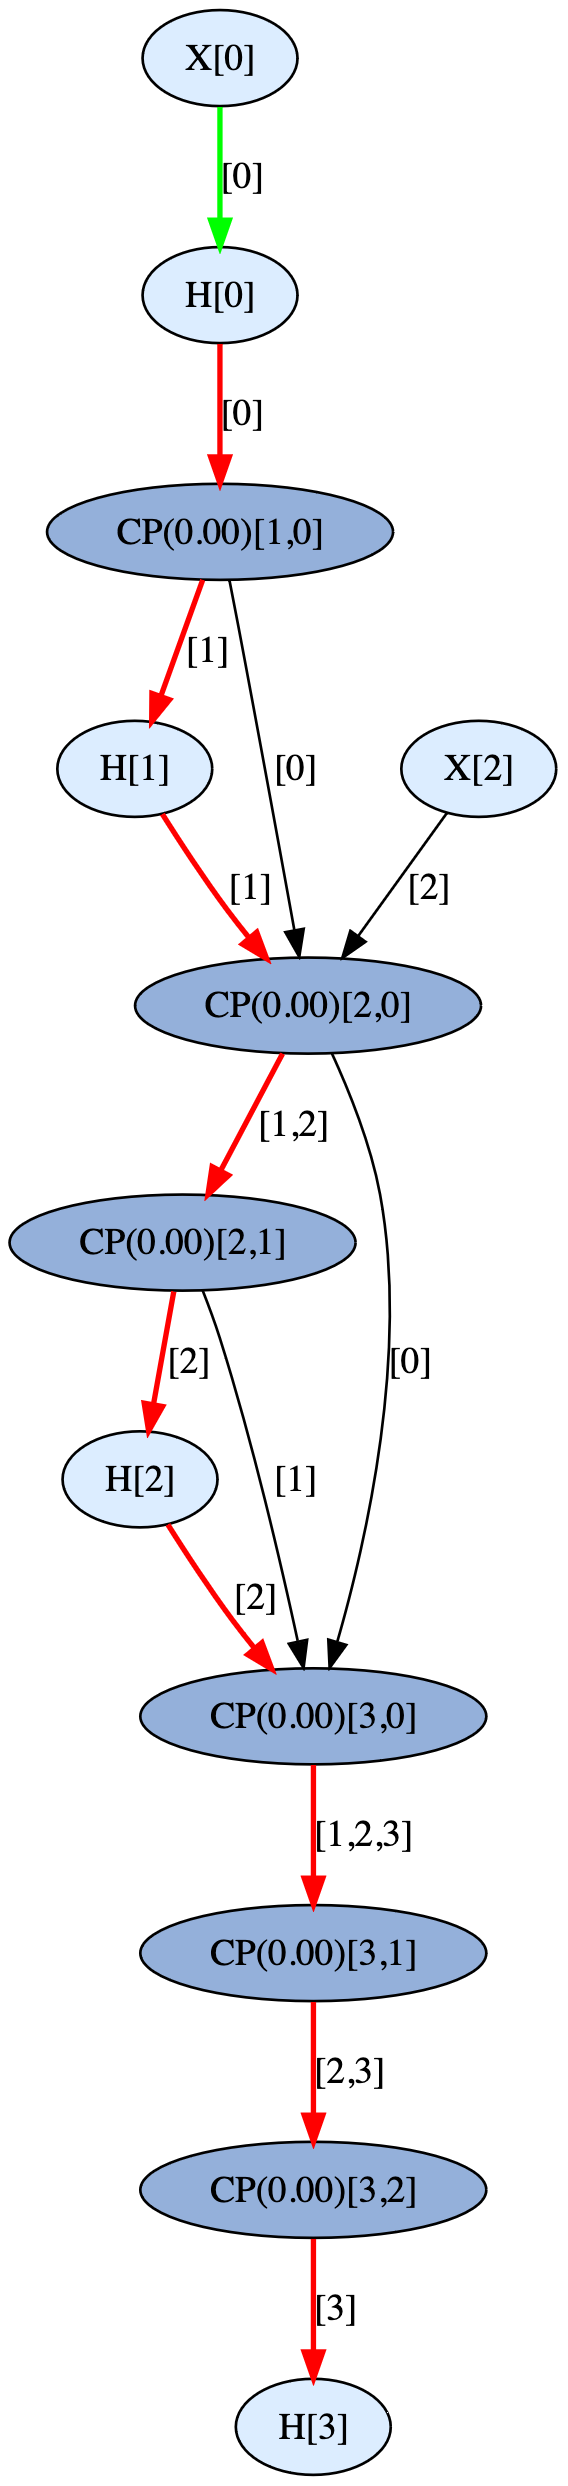
\includegraphics[width=.6\textwidth]{tensor_network.png}
        \caption{Tensor Network Representation of the QFT Circuit}
        \label{fig:tensor-network}
    \end{minipage}%
    \hfill
    \begin{minipage}{.45\textwidth}
        \centering
        \begin{tabular}{c}
            $\texttt{000: M(02x02)}\;\odot\;\texttt{M(02x02)}$ \\
            $\texttt{001: I(00000)}\;\otimes\;\texttt{M(02x02)}$ \\
            $\texttt{002: I(00001)}\;\odot\;\texttt{M(04x04)}$ \\
            $\texttt{003: M(02x02)}\;\otimes\;\texttt{M(02x02)}$ \\
            $\texttt{004: I(00002)}\;\odot\;\texttt{I(00003)}$ \\
            $\texttt{005: I(00004)}\;\otimes\;\texttt{M(02x02)}$ \\
            $\texttt{006: M(04x04)}\;\otimes\;\texttt{M(02x02)}$ \\
            $\texttt{007: I(00006)}\;\odot\;\texttt{M(08x08)}$ \\
            $\texttt{008: I(00005)}\;\odot\;\texttt{I(00007)}$ \\
            $\texttt{009: M(02x02)}\;\otimes\;\texttt{M(02x02)}$ \\
            $\texttt{010: M(04x04)}\;\odot\;\texttt{I(00009)}$ \\
            $\texttt{011: M(02x02)}\;\otimes\;\texttt{I(00010)}$ \\
            $\texttt{012: I(00008)}\;\odot\;\texttt{I(00011)}$ \\
            $\texttt{013: I(00012)}\;\otimes\;\texttt{M(02x02)}$ \\
            $\texttt{014: M(02x02)}\;\otimes\;\texttt{M(08x08)}$ \\
            $\texttt{015: M(16x16)}\;\odot\;\texttt{I(00014)}$ \\
            $\texttt{016: M(02x02)}\;\otimes\;\texttt{M(02x02)}$ \\
            $\texttt{017: M(04x04)}\;\odot\;\texttt{I(00016)}$ \\
            $\texttt{018: M(04x04)}\;\otimes\;\texttt{I(00017)}$ \\
            $\texttt{019: I(00015)}\;\odot\;\texttt{I(00018)}$ \\
            $\texttt{020: I(00013)}\;\odot\;\texttt{I(00019)}$
        \end{tabular}
        \caption{Operation Plan for the QFT Circuit}
        \label{fig:operation-plan}
    \end{minipage}
\end{figure}

\begin{figure}
    \centering
    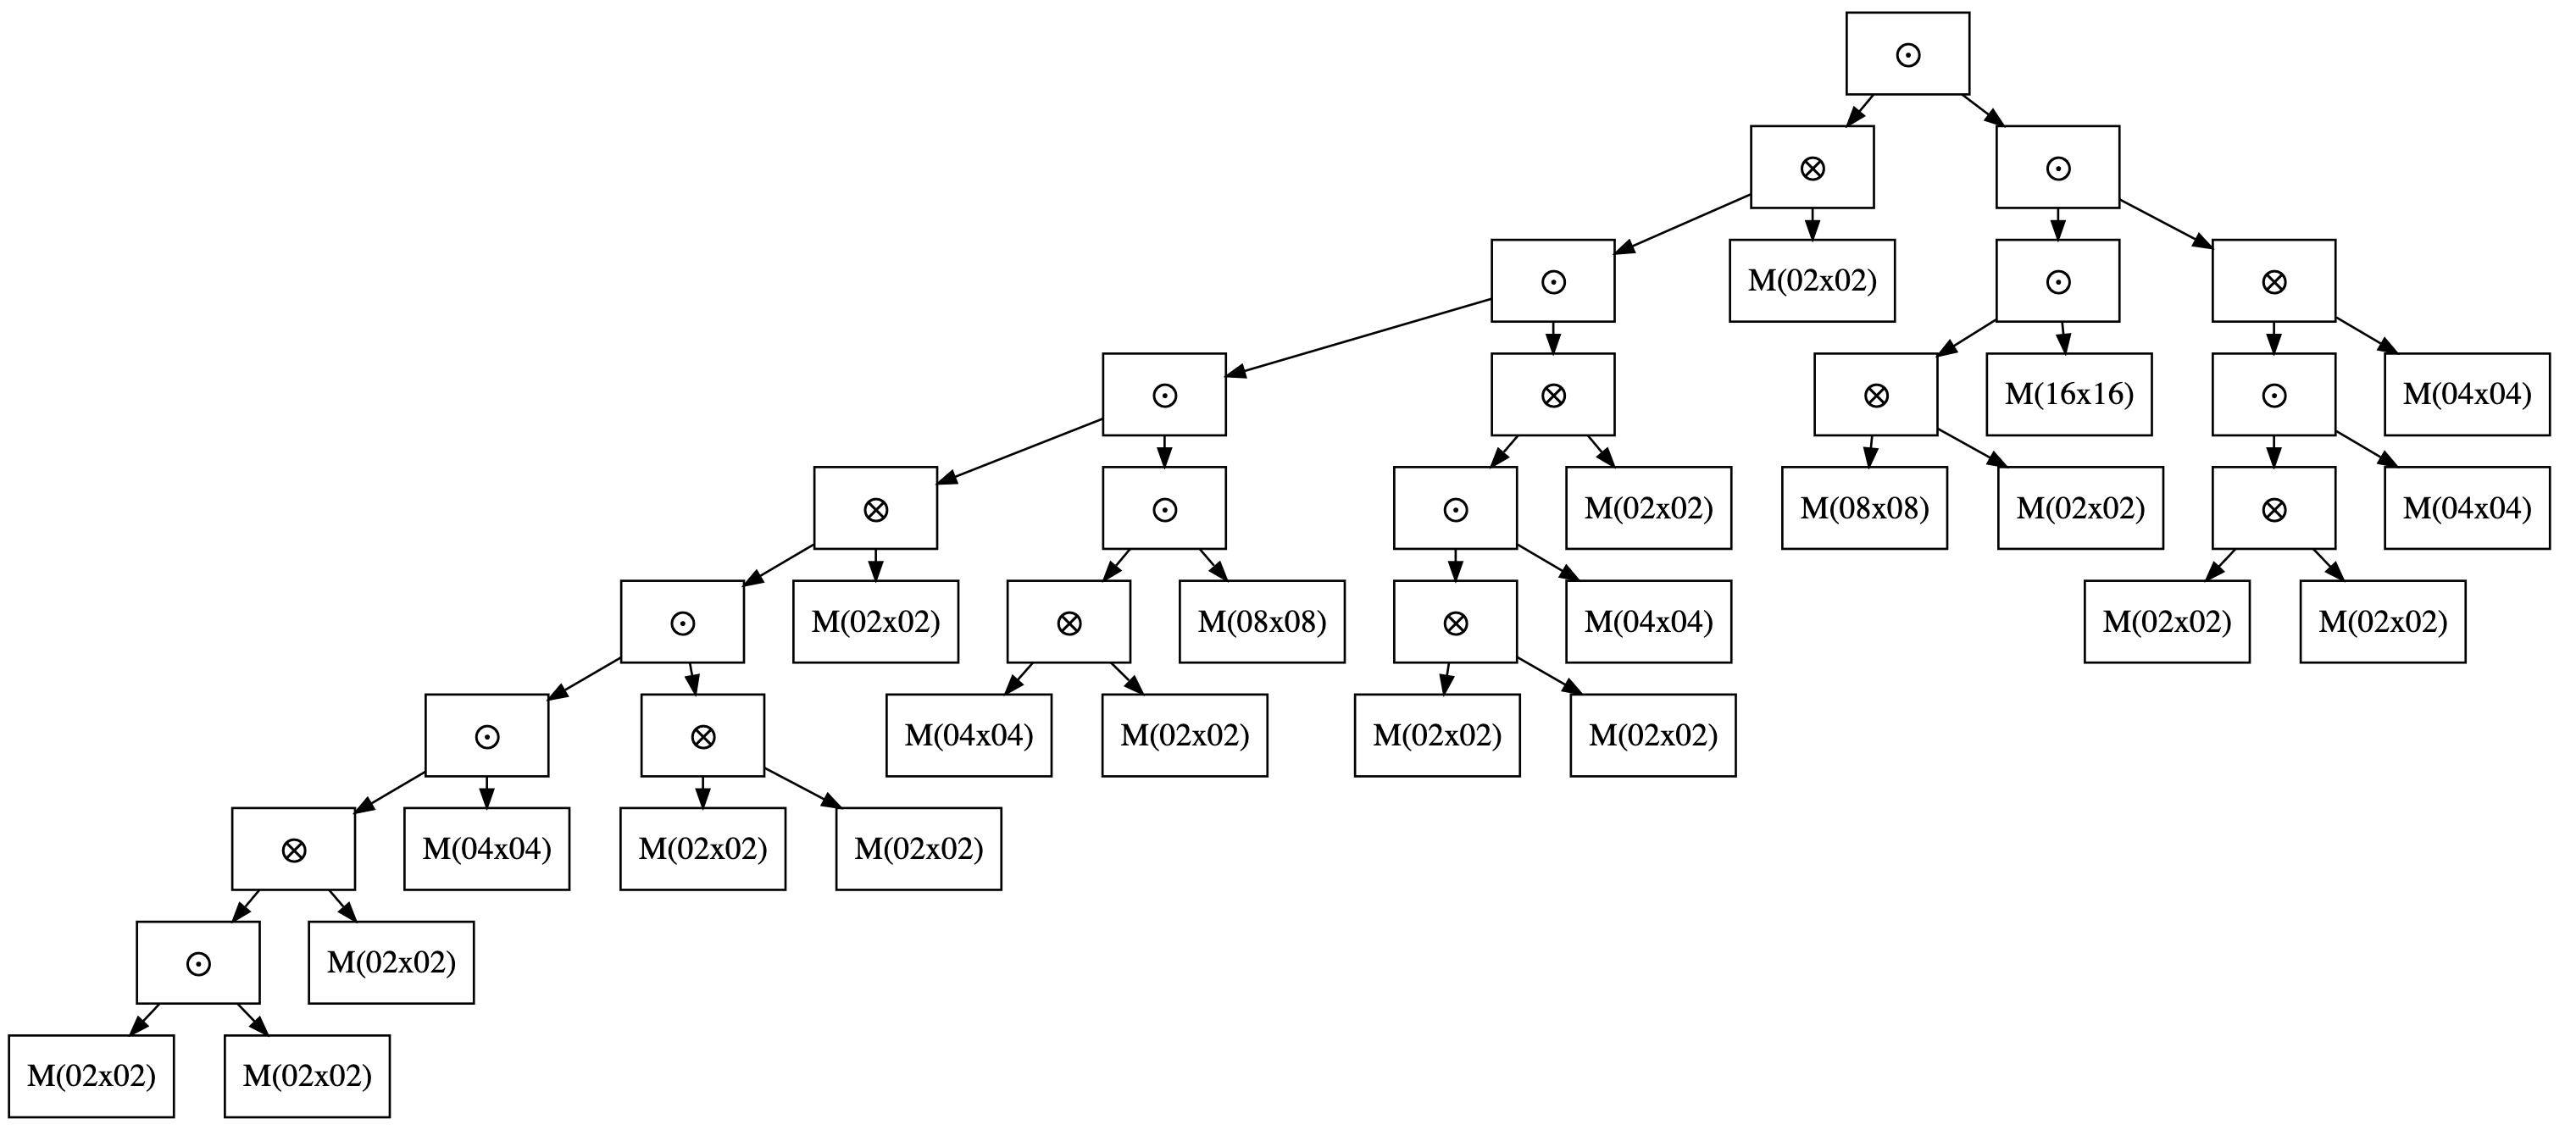
\includegraphics[width=\textwidth]{operation_tree.png}
    \caption{Operation Tree for the QFT Circuit}
    \label{fig:operation-tree}
\end{figure}

Highlighted in green is the contraction that will be performed first, as it has the lowest cost (rank 1, involving only 1 qubit). The contractions highlighted in red will be re-evaluated in another \textbf{sweep} of the algorithm, that is the process of identifying the optimal contraction path.

Starting from the tensor network, the frontend will go through a series of intermediate steps, eventually leading to the generation of an \textbf{Operation Tree} (OT) (figure~\ref{fig:operation-tree}) and its subsequent \textbf{Operation Plan} (Op) (figure~\ref{fig:operation-plan}). This plan is fed to the scheduler, that will optimize the order of the operations to send to the backend for execution.

Each instruction can be seen as a tensor operation, with the format:

\begin{center}
    \texttt{<ID>: <T1> <OP> <T2>}
\end{center}

Where \texttt{<ID>} is the instruction identifier, \texttt{<T1>} and \texttt{<T2>} are the tensors involved in the operation, and \texttt{<OP>} is the operation to be performed (e.g., $\otimes$ for tensor expansion and $\odot$ for matrix multiplication). The tensor operands can be identified either directly by matrix dimensions or by the address, if the the operation has a dependency on a previous instruction.

\FloatBarrier

\subsubsection{Future Work and Optimizations}

While the current implementation provides a robust foundation, several areas for future improvement have been identified:

\begin{itemize}
    \item Extending QASM support to full specification compliance
    \item Optimizing the contraction tree generation algorithm employing advanced graph based techniques \cite{PhysRevE}
    \item Implementing and optimizing the OpenCL communication layer for FPGA and GPU backends
    \item Exploring advanced scheduling techniques for improved instruction-level parallelism
\end{itemize}

Potential optimization strategies include the implementation of a hybrid CPU-FPGA approach for dynamic workload distribution and the exploration of quantum-inspired classical algorithms for improved tensor network contraction.

By continually refining and expanding the frontend's capabilities, we aim to create a versatile and efficient quantum circuit simulation framework that can leverage various backend architectures and implementations.

\subsection{Instruction Set Architecture (ISA) Design}
\label{subsec:isa}

An Operation Plan (OP) can be compiled into a set of instructions described better in the following table:

\begin{table}[t]
	\caption{ISA for computations on the FPGA backend}
	\centering
	\resizebox{.7\textwidth}{!}{\begin{tabular}{cccc}
		\toprule
		\textbf{Instruction} & \textbf{Opcode} & \textbf{Left Operand} & \textbf{Right Operand}\\
		\midrule
		\texttt{TE(MxM)} & \texttt{0x01} & \texttt{CooMatrixFmt} & \texttt{CooMatrixFmt} \\
        \texttt{TE(MxA)} & \texttt{0x02} & \texttt{CooMatrixFmt} & \texttt{AddressFmt} \\
        \texttt{TE(AxM)} & \texttt{0x03} & \texttt{AddressFmt} & \texttt{CooMatrixFmt} \\
        \texttt{TE(AxA)} & \texttt{0x04} & \texttt{AddressFmt} & \texttt{AddressFmt} \\
        \texttt{MM(MxM)} & \texttt{0x05} & \texttt{CooMatrixFmt} & \texttt{CooMatrixFmt} \\
        \texttt{MM(MxA)} & \texttt{0x06} & \texttt{CooMatrixFmt} & \texttt{AddressFmt} \\
        \texttt{MM(AxM)} & \texttt{0x07} & \texttt{AddressFmt} & \texttt{CooMatrixFmt} \\
        \texttt{MM(AxA)} & \texttt{0x08} & \texttt{AddressFmt} & \texttt{AddressFmt} \\
		\bottomrule
	\end{tabular}}
	\label{tab:isa}
\end{table}

The Instruction Set Architecture (ISA) described in table~\ref{tab:isa} is designed to support the execution of tensor expansion (\texttt{TE}) and matrix multiplication (\texttt{MM}) operations on the FPGA backend. The ISA defines a set of opcodes that correspond to specific tensor operations, each with distinct operand formats. The operands are represented in custom formats:

\begin{itemize}
    \item \texttt{CooMatrixFmt}: Represents a matrix in Coordinate (COO) sparse format, containing non-zero values and their corresponding row and column indices. To see the full definition of the format, refer to the table~\ref{tab:coo-matrix-fmt}.
    \item \texttt{AddressFmt}: Represents the memory address of a matrix in the FPGA memory space, by encoding a single 32-bit address in little-endian format.
\end{itemize}

\begin{table}
    \caption{COO Matrix Format}
    \centering
    \resizebox{.9\textwidth}{!}{\begin{tabular}{lcc}
        \toprule
        \textbf{Value} & \textbf{Format} & \textbf{Amount} \\
        \midrule
        number of non zero elements (\texttt{NZ}) & \texttt{uint32\_t} & \texttt{1} \\
        rank of the tensor & \texttt{uint8\_t} & \texttt{1} \\
        format (col-major or row-major) & \texttt{uint8\_t} & \texttt{1} \\
        element value & \texttt{CooElementFmt~\ref{tab:coo-el-fmt}} & \texttt{NZ} \\
        \bottomrule
    \end{tabular}}
    \label{tab:coo-matrix-fmt}
\end{table}


\begin{table}
    \caption{COO Element Format}
    \centering
    \resizebox{.5\textwidth}{!}{\begin{tabular}{lcc}
        \toprule
        \textbf{Value} & \textbf{Format} & \textbf{Amount} \\
        \midrule
        row index & \texttt{uint32\_t} & \texttt{1} \\
        column index & \texttt{uint32\_t} & \texttt{1} \\
        real & \texttt{float} & \texttt{1} \\
        imaginary & \texttt{float} & \texttt{1} \\
        \bottomrule
    \end{tabular}}
    \label{tab:coo-el-fmt}
\end{table}

\FloatBarrier

\subsection{Backend}

% TODO - extensive use of producer-consumer pattern in kernel design
This section provides an in-depth overview of the FPGA backend, focusing on the architectural design and optimization strategies employed in kernel design. Since the development of both the FPGA kernels has been done from scratch, after months of research and development devoted to the development and optimization of the frontend, the backend currently lacks the same level of maturity and polish. However, being the FPGA backend a crucial component of the toolchain, we focused on delivering a functional prototype that can be further refined and optimized in future iterations.

\subsubsection{Architectural Overview}

Our FPGA-based acceleration solution comprises two primary kernels, each tailored for a specific mathematical operation described in the ISA previously presented:

\begin{enumerate}
    \item \textbf{Tensor Expansion Kernel}: Implements the Kronecker product operation between two sparse (COO) matrices of variable dimensions, used in tensor expansion operations.
    \item \textbf{Matrix Multiplication Kernel}: Performs sparse (COO) matrix multiplication for tensor contractions.
\end{enumerate}

Both kernels are designed to operate on matrices represented in the Coordinate (COO) sparse format, meeting strict memory constraints and ensuring efficient memory access patterns. Choosing the right sparse format is fundamental for a feasible FPGA implementation\cite{FormatsHwSpMsurvey}, as it allows for reduced memory bandwidth requirements and improved computational density, at the cost of dynamic and imperfect loop structures. Choosing COO format allows the kernels to be used transparently with both row-major and column-major matrices, by simply changing the order of the elements in the input stream. The advantages of this approach will be further discussed in the following sections.

\subsubsection{Implementation Details}
% TODO Provide detailed explanations of the implementation using Vitis HLS. Discuss any optimizations made for performance.

% - no external libraries used, only Vitis HLS includes
% - use of vitis as the main tool for kernel development
The kernels have been implemented from scratch using Vitis High-Level Synthesis (HLS), without relying on external libraries beyond the standard Vitis HLS includes. This approach allows for fine-grained control over the hardware implementation and optimization strategies.

\subsubsection{Tensor Expansion Kernel}

The Tensor Expansion kernel implements the Kronecker product of two arbitrarily large matrices. This operation is fundamental to the tensor product operations in quantum circuit simulation.

Key features of the Tensor Expansion kernel include:

% - tensor expansion kernel
% 	- kronecker product of an arbitrary large matrix with another large arbitrary matrix
% 	- employed for the tensor product operation in the tensor network contraction
%   - use of a customized binary data format to read operations from a file and feed them to the kernel
\begin{itemize}
    \item Support for arbitrary matrix dimensions, accommodating various quantum gate configurations.
    \item Efficient handling of sparse matrices in COO format, minimizing memory bandwidth requirements.
    \item Utilization of the dataflow pragma for enhanced pipelining and parallelism.
\end{itemize}

\subsubsection{Matrix Multiplication Kernel}

The Matrix Multiplication kernel performs the multiplication of two sparse matrices in COO format, which is essential for tensor contraction operations in the quantum circuit simulation process. In particular, we leverage the usage of the matrix transposition to make sure that both the tensors are fed to the kernel in the correct order, in particular the left tensor is fed by rows while the right tensor is fed by columns.

Notable aspects of the Matrix Multiplication kernel include:

% - matrix multiplication kernel
% 	- multiplication of two sparse matrices in COO format
% 	- employed for the tensor contraction operation in the tensor network contraction
%   - use of packet based approach to handle the sparse matrix multiplication
\begin{itemize}
    \item Implementation of a packet-based approach to efficiently handle sparse matrix multiplication. In particular, the kernel allows for read packets of non-zero values specified by the preprocessor directive PACKET_SIZE.
    % imperfect loop due to the nature of the problem (employing COO format)
    \item Optimization for the inherently imperfect loop structures resulting from the COO format. This is because the storage method of the matrix guarantees that multiplication for zero values are avoided, so we just need to check the indexes on the non zero ones (all the ones present in the coo stream) and appropriately update the accumulator for each element of the output tensor.
    \item Extensive use of the producer-consumer pattern to enhance data flow and reduce latency. This is done to maximize the efficiency of the dataflow pattern which feeds data to the fpga, it get quantised and used to compute the result. In particular, there is a double producer-consumer pattern; this is due to the fact that we perform the computation of the results in row major, and thus to guarantee an in-order result stream, we need to consume and temporarily store each row of the left tensor, while it gets multiplied by the entire right tensor. Likewise, we need to consume and produce the entire B tensor for each row that multiplies it.
\end{itemize}

\subsubsection{Optimization Strategies}

Several optimization techniques have been employed to maximize the performance of our FPGA kernels:

\begin{enumerate}
    \item \textbf{Dataflow Optimization}: Extensive use of the dataflow pragma enables pipelining and parallelism, significantly improving throughput.

    \item \textbf{Memory Access Optimization}: The COO sparse matrix format reduces memory bandwidth requirements, crucial for handling large quantum circuits.

    \item \textbf{Packet-Based Processing}: Implemented in the Matrix Multiplication kernel to efficiently handle sparse data structures and improve computational density.

    \item \textbf{Producer-Consumer Pattern}: This design pattern enhances data flow between different stages of the computation, reducing overall latency.
\end{enumerate}

\subsubsection{Integration and Data Flow}
% Explain how the kernel integrates with the host side via OpenCL. Include diagrams and flowcharts to illustrate the process.
% - use of OpenCL for communication between the host and the FPGA
The integration of the FPGA kernels with the host side is facilitated through OpenCL, enabling efficient communication and data transfer between the host CPU and the FPGA device.

% \begin{figure}[h]
%     \centering
%     % Replace with actual path to your diagram
%     \includegraphics[width=0.8\textwidth]{path_to_your_diagram}
%     \caption{Data flow between Host and FPGA Kernels}
%     \label{fig:dataflow}
% \end{figure}

% - use of dataflow pragma for pipelining and parallelism
The data flow process can be summarized as follows:

\begin{enumerate}
    \item The host prepares input data in a custom binary format, encoding the operations to be performed.
    \item This data is transferred to the FPGA device memory via OpenCL.
    \item The appropriate kernel (Tensor Expansion or Matrix Multiplication) is invoked to process the data.
    \item Results are transferred back to the host for further processing or final output.
\end{enumerate}

\subsubsection{Code Example: Tensor Expansion Kernel}
% Include HLS code snippets and explain their functionality.

To illustrate the implementation details, consider the following simplified code snippet from the Tensor Expansion kernel:

This snippet demonstrates the use of HLS pragmas for interface specification and dataflow optimization, as well as the division of the kernel into separate read and compute stages for improved pipeline efficiency.

\subsubsection{Performance Considerations}

The performance of our FPGA-based solution is influenced by several factors:

\begin{itemize}
    \item \textbf{Memory Bandwidth}: The efficiency of data transfer between off-chip memory and on-chip processing elements.
    \item \textbf{Computational Density}: The ratio of compute operations to memory operations, which is optimized through our packet-based approach.
    \item \textbf{Parallelism}: The degree of concurrent execution achieved through our dataflow design and kernel architecture.
    \item \textbf{Precision}: The use of fixed-point arithmetic (\texttt{ap\_fixed<16,8>}) balances computational accuracy with hardware resource utilization.
\end{itemize}

\subsubsection{Future Work and Optimizations}

While the current implementation provides a solid foundation for FPGA-accelerated quantum circuit simulation, several areas for future enhancement have been identified:

\begin{enumerate}
    \item Implementation of multiple Processing Elements (PEs) for the sparse matrix multiplication kernel to further increase parallelism.
    \item Exploration of dynamic indexing schemes for the Tensor Expansion kernel to improve flexibility and efficiency for varying input sizes.
    \item Investigation of mixed-precision arithmetic to optimize the trade-off between accuracy and performance.
    \item Development of a more sophisticated OpenCL-based communication layer to enable dynamic scheduling and workload distribution between the host and FPGA.
\end{enumerate}

By continuing to refine and optimize our FPGA kernel implementations, we aim to push the boundaries of what's possible in hardware-accelerated quantum circuit simulation, providing a powerful tool for researchers and practitioners in the field of quantum computing.




%%%%%%%%%%%%%%%%%%%%%%%%%%%%%%%%%%%%%%%%%%%%%%%%%%%% SECTION 4

\section{Results}
\label{sec:results}

\subsection{Setup}
% what was run and on which architecture (to allow others to replicate results)
- tests in local:
	- clone repo
	- install cmake, just and other requirements
	- ... run tests, look at justfile or type just into terminal
- vitis hls
	- which version
	- ...
- vivado/opencl
	- version
	- parameters to compile kernel (clock frequency, board - alveo u55c, ...)
	- ...

\subsection{Results and comparisons}

% FIXME change name
\subsubsection{Single times}
\subsubsection{Total time end to end}
	- only cpu
	- only fpga

Notes:
	- highlight kernels are proof of concepts
	- add and highlight isa
	(I THINK IT CAN BE VERY IMPORTANT) highlight situations in which engineering tradeoff had to be made, what was the domain, the requirements, the final decision and the considerations that lead to it.





%%%%%%%%%%%%%%%%%%%%%%%%%%%%%%%%%%%%%%%%%%%%%%%%%%%% REFERENCES

\printbibliography[title={\section{References}}]

%%%%%%%%%%%%%%%%%%%%%%%%%%%%%%%%%%%%%%%%%%%%%%%%%%%% APPENDICES
\section{Appendices}
An explanation of some technical terms used in the report.
- bitstring : in quantum computing, it refers to
- gate : in a quantum circuit,
- lane :
- sota : state of the art
- state vector : in a quantum circuit,
- tensor : math object that
- tensor expansion : math operation that


\end{document}
